% !TEX spellcheck=en_US
\documentclass[a4paper]{article}
\usepackage[american]{babel}
\usepackage[T1]{fontenc}
\usepackage[utf8]{inputenc}
\usepackage[activate={true,nocompatibility},final,tracking=true,kerning=true,spacing=true,factor=1100,stretch=10,shrink=10]{microtype}
\usepackage{graphicx}
\usepackage{csquotes}
\usepackage{hyperref}
\usepackage{url}
\usepackage[backend=biber,style=ieee]{biblatex}

% misc macros
\newcommand*{\pref}[2]{#1 (\ref{#2})}

% microtype
\SetTracking{encoding={*}, shape=sc}{0}

\addbibresource{bibliography.bib}

\begin{document}

\begin{titlepage}
    \centering
    {\scshape\Huge \bfseries{Advanced Systems} \par}
    \par\vspace{1cm}
    
\includegraphics[width=0.45\textwidth]{images/LLVM_Logo.png}\par
    \vspace{3cm}
    {\huge\bfseries The C++ Build Process \par}
    \vspace{1cm}
    {\LARGE\itshape Shinonome Mazawa \par}
    \vspace{1cm}
    {\large\today\par}
    \vfill
    \begin{abstract}
        If you're a beginner and started to learn C++ very recently, read the chapters
        Preprocessor, Compiler, Linker, and Conclusions first. For the most part,
        all definitions and explanations in these chapters are compiler-independent.
        Come back to this document later after you moved on from writing terminal
        applications exclusively. The remaining chapters provide additional information
        by example of LLVM/Clang. See also the Appendix and Bibliography for further
        reading. 
    \end{abstract}
\end{titlepage}

\newpage

\microtypesetup{protrusion=false}
\tableofcontents
\microtypesetup{protrusion=true}

\newpage

% === Begin Section Includes ===

\section{Introduction}

When it comes to literature, a common distinction is made between three major 
forms that are of great interest, namely poetry, prose and drama. By way of 
an introduction, we are going to take a look at the terminology below to help 
us set the stage for the upcoming discussion. What follows is a brief breakdown 
of a selection of books that changed the world of literature forever. Originally
intended to serve as an introduction to an essay that explores past and future 
of Japanese Light Novels, the books mentioned here encouraged me to go a little 
more into depth about the authors responsible for the early English novels. This
will prove important later when we embark on an adventure through the world of 
Light Novels in search of distinct characteristics and influences.


\section{Preprocessor}

A preprocessor directive uses the pound character (\path{#}) to designate a
preprocessor statement. These directives give rise to various events, such as

\begin{itemize}
    \item file inclusion (\path{#include}) in which the file being processed
    incorporates the content of another file.
    \item macro substitution (\path{#define}) to denote a sequence of text that
    is to be replaced by a definition.
    \item preprocessor directives (\path{#ifdef} or\footnote{These two are not
    exactly the same, see also \url{https://stackoverflow.com/questions/135069}.}
    \path{#if defined}) for introducing conditions under which segments of code
    shan't compile\footnote{This directive is primarily used for header guards,
    but it can also be used to denote sections in code that are specific to the
    operating system, for example \path{#if defined(__ANDROID__)}.}. 
\end{itemize}

The preprocessor takes precedence over the compiler. Once this step is executed,
all preprocessor directives are removed from the source file. Files that go through
this translation process turn into translation units that only exist in memory.

\section{Compiler}

Creating a binary executable from C++ code is a multistage process that can be
divided into two major steps: compiling and linking. Each of these steps goes
through a magnitude of sub-routines whose end goal is to produce a binary executable
file that is used to run the main application. Alternatively, compilers are also
capable of creating a static or shared library that can be used in other projects.
Prominent examples include, amongst other things:

\begin{itemize}
    \item \textbf{Boost:} a set of 164 individual libraries that range from Algorithm
    to YAP, an expression template library for C++14 and later.
    \item \textbf{STL:} a standard template library.
    \item \textbf{QT:} a tried-and-tested template library.
    \item \textbf{SFML:} a simple and fast multimedia library living up to its name.
    \item \textbf{OpenCV:} a high-performance image processing library.
\end{itemize}

There are many C++ compilers out there, but the ones most commonly used probably are:

\begin{itemize}
    \item Clang
    \item GCC
    \item MSVC
    \item Intel C++ Compiler
\end{itemize}

The main purpose of a compiler is to translate a high-level language into a transient
lower-level language, for example assembly. In \autocite{wirth1996}, a compiler is
defined as a program that automatically translates a program text into a suitable
instruction sequence before it is processed by a computer where the text to be
translated is called source code (or sometimes source text). Note that some compilers
don't use an assembler in an intermediate step at all, but rather directly emit
byte code into an object file. In the simplest terms, an object file consists of
three things:

\begin{itemize}
    \item Ranges of unsplittable data (sections and atoms)
    \item Names that define or reference data (symbols)
    \item Lists of modifications to data (relocations)
\end{itemize}

In many cases the compiler is able to produce more efficient assembly code than
if it were handwritten. One of its main responsibilities is to ensure that the code
follows the rules of the C++ programming language. During this step the compiler
also performs a series of optimization techniques where applicable (inter alia
constant folding and function inlining) before the assembler transforms this intermediate
product into object code. Bear in mind that many compilers turn off all optimizations
by default to improve the debug experience. They're the penultimate result of the
build process and contain machine code with unresolved external dependencies that
are fed into the linker in the next stage. Some compilers provide support for multiple
languages or target architectures which is one of the many compelling reasons to
use them over others. In comparison, a traditional static compiler uses a three-phase
design whose major components are the frontend, optimizer and the backend \autocite{lattner2011}.

\begin{itemize}
    \item \textbf{Frontend:} Performs lexical and syntax analysis as well as type
    checking, the result of which is the abstract syntax tree (AST) that represents
    the structure of the source text.
    \item \textbf{Optimizer:} Derives information from the intermediate code
    representation (IR) in order to recognize instructions that can be replaced
    with functionally equivalent optimizations.
    \item \textbf{Backend:} Generates machine-dependent optimizations (for example
    peephole optimizations in assembly). This code targets a specific CPU architecture. 
\end{itemize}

\begin{figure}[hbt!]
    \centering
    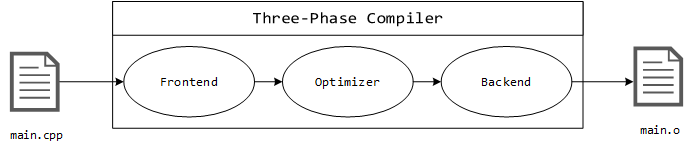
\includegraphics[width=1\textwidth]{images/ThreePhaseDesign.png}
\end{figure}

LLVM takes this design to the next level by implementing a modular compiler system
that provides an interface for many different languages. The advantage of this design
is the common optimizer that can be repurposed for different compiler frontends,
while also redirecting development efforts into a single component which further
increases the quality of the compiler that is now backed by a larger community.

\begin{figure}[hbt!]
    \centering
    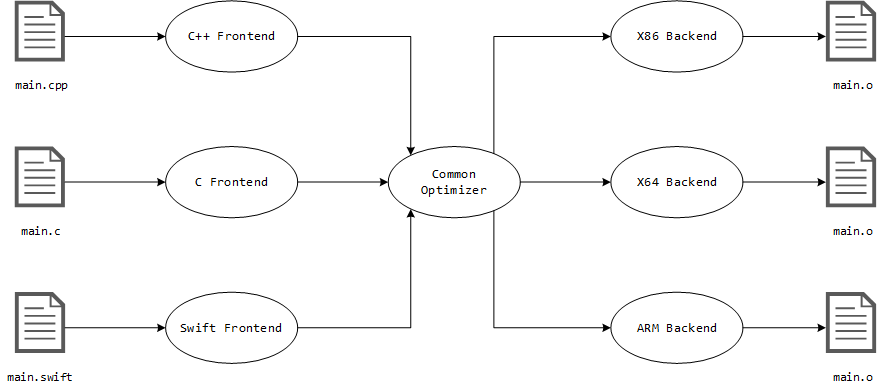
\includegraphics[width=1\textwidth]{images/ThreePhaseDesignRetargeting.png}
\end{figure}

There are other reasons why commercial application developers would prefer LLVM
over other compilers such as GCC: it is licensed under a BSD-style Apache License
v2.0 as opposed to GCC v4.3+ which uses the less permissive copyleft GPLv3 license
that is not viable for propriety projects \autocite{fandrey2010}. However, this is
not the decisive factor for small applications written by independent developers
or students. In many cases, using the GPLv3 license for a project would be more
beneficial for the open-source software community\footnote{For a more thorough
explanation visit \url{https://www.gnu.org/licenses/rms-why-gplv3.html}.}.

Most compilers provide a set of increasingly performant optimization options that
can be controlled by explicitly enabling their respective flags. Starting with v11.0,
Clang has changed its optimization flags to match the defaults of GCC. In case of
Clang, it defines these flags as followed\footnote{See also this \url{https://clang.llvm.org/docs/CommandGuide/clang.html}
for a comprehensive list of command line options.}:

\begin{itemize}
    \item \texttt{-O0:} On this level, no optimization pass is enabled. It compiles
    the fastest and generates the most executable code.
    \item \texttt{-O1:} Somewhere between \texttt{-O0} and \texttt{-O2}.
    \item \texttt{-O2:} Moderate level of optimization which enables most optimizations.
    \item \texttt{-O3:} Like \texttt{-O2}, except that it enables optimizations
    that take longer to perform or that may generate larger code (in an attempt
    to make the program run faster).
    \item \texttt{-Ofast:} Enables all the optimizations from \texttt{-O3} along
    with other aggressive optimizations that may violate strict compliance with
    language standards.
    \item \texttt{-Os:} Like \texttt{-O2}, with extra optimizations to reduce code size. 
    \item \texttt{-Oz:} Like \texttt{-Os} (and thus like \texttt{-O2}) but reduces
    code size further.
    \item \texttt{-Og:} Like \texttt{-O1}. In future versions, this option might
    disable different optimizations in order to improve debuggability.
    \item \texttt{-O:} Equivalent to \texttt{-O1}.
    \item \texttt{-O4:} Currently equivalent to \texttt{-O3}.
\end{itemize}

Building projects for release purposes is a whole topic on its own and is not going
to be covered in this document in any more detail. 


\section{Linker}

The final element in the chain of the build process is the linker. It takes the
object files that were produced by the compiler in the previous step and resolves
all symbols in other files.

On a related note, an important term that often appears in this context is the word
linkage. A distinction is drawn between internal and external linkage. Internal
linkage refers to any identifier whose accessibility is limited to a single
translation unit. By contrast, external linkage refers to any identifier that is
accessible by other translation units via a forward declaration.

At first glance it might seem strange to separate the compilation process from
the linker. But there are several advantages to this design:

\begin{itemize}
    \item A modular design enables the compiler to work with different but
    compatible linkers.
    \item The implementation complexity of the compiler is possibly reduced if both
    steps are distinct from each other (e.g., during compilation it can assume that
    a function is defined in another file).
    \item Because the linker springs into action as a post-compilation process,
    modifying a single header file does not necessarily induce the re-compilation
    of all project files (with the exception of any file that includes this header),
    one consequence of which is the fact is that the complete build process takes
    up less time.
    \item This distinction also enables multi-threaded compilation which further
    speeds up the build process.
\end{itemize}

On top of that there are more benefits to this approach. Understanding the difference
between compilation and linking makes it easier to interpret bugs in code. Error
messages often indicate at which stage an error was detected:

\begin{itemize}
    \item \texttt{LNK2019: unresolved external symbol 'symbol' referenced in function 'function'.}
    \item \texttt{C2661: 'function': no overloaded function takes number arguments. }
\end{itemize}

In general, the compiler is capable of generating more precise error messages because
it has access to the abstract syntax tree (or an intermediate code representation
in case of Clang), which is why it can reason better about the code at hand. Therefore,
it is a good idea to write code in a way that any possible errors are caught by
the compiler rather than by the linker.

\begin{figure}[ht]
    \centering
    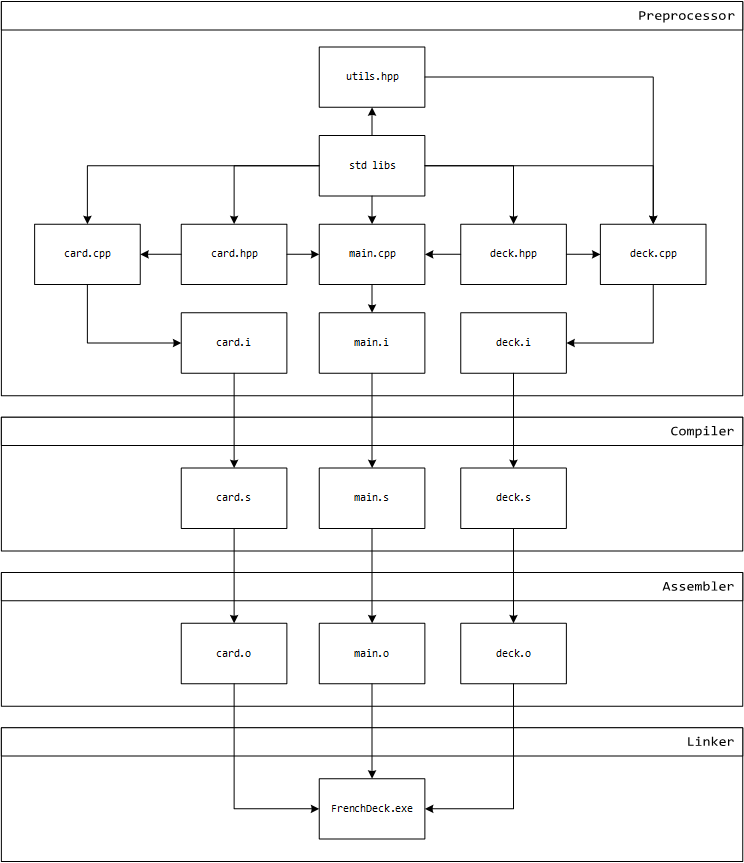
\includegraphics[width=1\textwidth]{images/FrenchDeck.png}
\end{figure}


\section{LLVM}

It is worth mentioning that there exist many compiler-specific preprocessor directives.
For portability reasons it is encouraged to avoid using them, though there is one
exception to this rule\footnote{Further reading: \url{https://en.wikipedia.org/wiki/Pragma_once}.}
(\path{#pragma once}). In general, a compiler is best thought of as a collection
of seven sequential phases, though in reality their implementation is more intertwined
than distinct from each other.

\begin{figure}[ht]
    \centering
    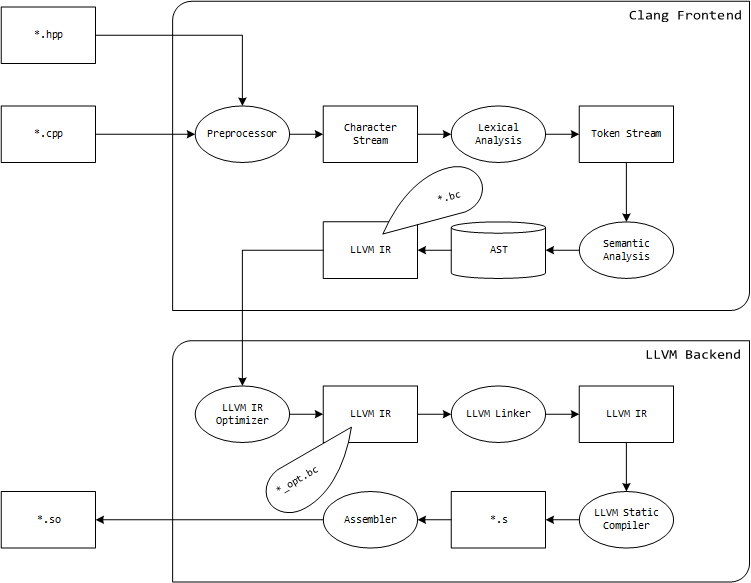
\includegraphics[width=0.8\textwidth]{images/LLVM.png}
\end{figure}

\begin{enumerate}
    \item \textbf{Preprocessing:} Evaluates all preprocessor directives (string
    concatenation) in memory and creates a character stream for further processing.
    \item \textbf{Lexical Analysis:} Reads and analyzes the incoming character
    stream by dividing it into tokens, each of which corresponds to a certain symbol
    in the source language (for example keywords, variable names or numbers). 
    \item \textbf{Syntax Analysis:} Parses the token stream and produces an abstract
    syntax tree that reflects the structure of the program.
    \item \textbf{Type Checking:} Examines the abstract syntax tree and determines
    if the program violates the semantic rules of the language (for example when
    a variable is used but not declared, or when a Boolean value is treated like
    a function pointer).
    \item \textbf{Intermediate Code Generation:} Translates the program into a
    machine-independent language (for example LLVM IR). This is also where most
    of the code optimization takes place.
    \item \textbf{Machine Code Generation:} Translates LLVM IR to assembly language
    for a specific machine architecture.
    \item \textbf{Assembly and Linking:} The assembler creates an object file,
    i.e., determines a binary representation and addresses of variables, function
    names, and so on \autocite{mogensen2010}.
\end{enumerate}

When the source language is also the implementation language\footnote{The language
the compiler itself is written in.} and the source text to be compiled is actually
a new version of the compiler itself, the process is called bootstrapping\footnote{This
is an advanced topic that is outside the scope of this document. For more information
see also: \url{https://en.wikipedia.org/wiki/Compiler-compiler}.} \autocite{grune2012}.
In case of C or C++ it is more appropriate to say that an ahead-of-time compilation
(AOT) takes place when the IR is lifted down to native machine code before the program
is executed. This is different from using a just-in-time (JIT) compiler in an alternative
implementation of Python.

LLVM IR is a RISC-like set of instructions that is capable of expressing statically
typed high-level language constructs with an infinite amount of function local
registers and is available in form of two file formats, bitcode (\texttt{.bc}) and
human-readable code (\texttt{.ll}). This intermediate code generation makes it
possible to link files that were originally written in different high-level languages,
such as C, C++, Go, Rust or Swift and enables efficient code optimization. At its
core, an IR module consists of three things: target information, global symbols
and miscellaneous other data.

\begin{figure}[ht]
    \centering
    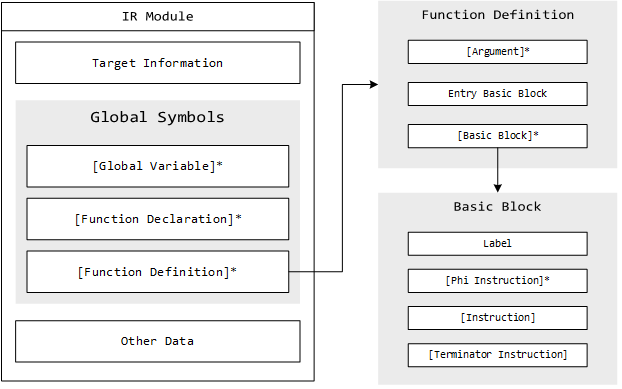
\includegraphics[width=0.7\textwidth]{images/LLVMIR.png}
\end{figure}

The target information starts with a pair of strings describing the target. For
example, the target layout string describes:

\begin{itemize}
    \item The endianness
    \item ELF mangling
    \item ABI alignment of i64
    \item Native integer widths
\end{itemize}

Moreover, the target triple string contains information about 

\begin{itemize}
    \item The architecture
    \item Vendor
    \item System
    \item ABI
\end{itemize}

A function definition, for instance, contains zero or more arguments, an entry
block as well as zero or more basic blocks. A basic block contains a label, zero
or more phi instructions, and zero or more instructions followed by the terminator
instruction. One of the main characteristics of a basic block is the control sequence:
it is written in SSA-form (Static Single Assignment), meaning that each register
is assigned exactly once which greatly simplifies control flow analysis. Phi
instructions return one value from a set of incoming values based on the control
flow path taken during execution to reach the phi instruction where each value is
associated with a predecessor basic block. An instruction performs arithmetic
operations or accesses the memory but doesn't alter the flow of the program. The
terminator instruction determines the control flow transfer once the basic block
finishes its execution. 


\section{Python Interpreter}

In order to obtain a thorough understanding of compilers, it is necessary to learn
how interpreters work and operate. By drawing this comparison between compilers and
interpreters it is possible to appreciate the benefits, but also acknowledge the
disadvantages both systems entail. By example of Python this section walks through
the design of an interpreter at a high-level which will be rounded up with a subsequent
evaluation in the next chapter.

At the highest level, the Python interpreter consists of two components: a compiler
that produces platform-independent bytecode, and the PVM (Python Virtual Machine)
which interprets and subsequentially executes the program. In addition to that,
the PVM accepts custom user input as well as pre-compiled library modules before
it goes over to execute the program.

\begin{figure}[ht]
    \centering
    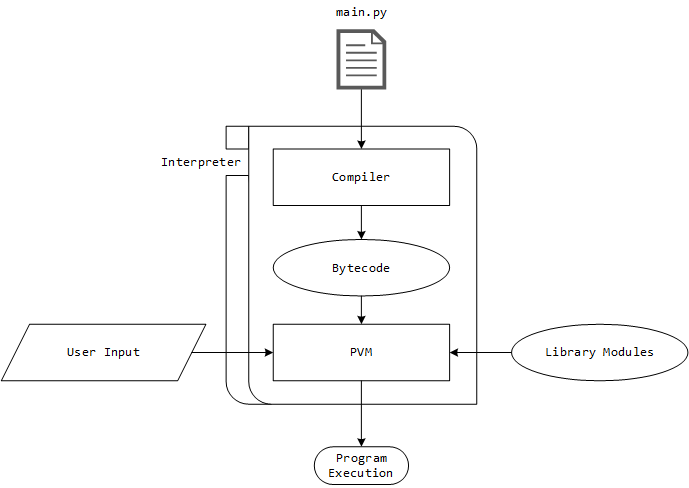
\includegraphics[width=0.7\textwidth]{images/BasicPythonArchitecture.png}
\end{figure}

At the second-highest level, the Python interpreter can be divided into three major
components: Parser, Compiler and PVM. Inside the parser, the scanner removes all
comments, white spaces, etc. to create a token stream that is passed on to the
Python parser, which in turn creates a parse tree. Note that the parse tree does
not contain any automated or symbolic connection between grammar specification and
the individual nodes in the parse tree. This parse tree is converted into an abstract
syntax tree by the AST converter. The AST is the highest-level representation of
the program structure where each AST node contains information about statements,
expressions, and several other specialized types like list comprehension and exception
handlers. The code generator takes the AST and translates it into a CFG (Control
Flow Graph) that can be thought of as an IR (intermediate representation) within
the blocks.

\begin{figure}[h]
    \centering
    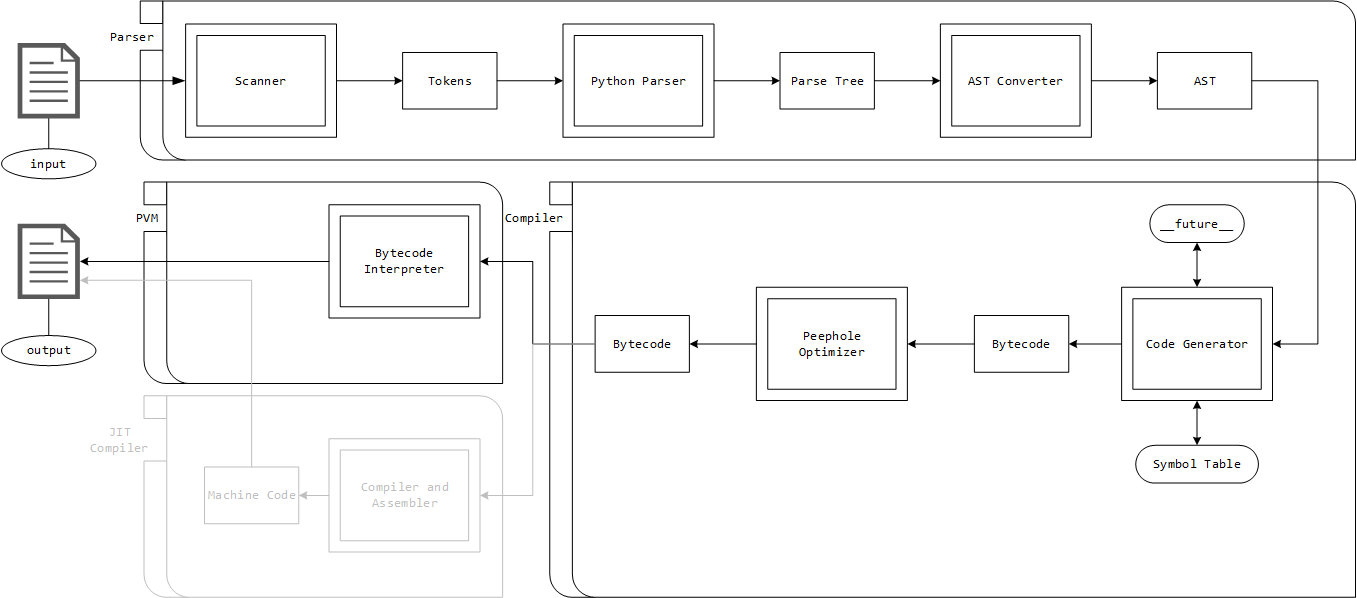
\includegraphics[width=1\textwidth]{images/PythonArchitecture.png}
\end{figure}

Basic blocks themselves are a block of IR with one entry point (that is the target
of something with the potential of changing the control flow) and possibly multiple
exit points which can change the flow of the program by using jumps or return
statements. Bytecode is generated directly from the CFG by doing a post-order
depth-first search on the CFG following the edges. After that the bytecode goes
through the peephole optimizer before it enters the PVM. From then on, there are
two possible paths that can be taken before the program execution takes place:

\begin{enumerate}
    \item CPython is the reference implementation of the Python programming language
    which utilizes a bytecode interpreter to trigger the program execution.
    \item Alternative language implementations (such as Numba\footnote{Numba is
    an open-source JIT compiler that translates a subset of Python and NumPy code
    into machine code by using the LLVM compiler library.}, PyPy\footnote{Uses an
    interpreter written in RPython and a JIT compiler to translate the source code
    into machine code instructions.}, or IronPython\footnote{Targets Microsoft's
    .NET framework and uses its JIT compiler to improve the program execution time.
    This implementation also removes the python's built-in GIL (Global Interpreter
    Lock).}, employ a JIT compiler to reduce the overhead that is caused by the
    interpreter by translating the bytecode into machine code instructions which
    often improves the performance of the program significantly.
\end{enumerate}

In CPython, memory is pooled in a single location for easy allocation and removal.
Because memory allocation for all needed memory in the compiler registers that memory
with the arena, a single call to free the arena is all that is needed to completely
free all memory used by the compiler \autocite{python2021}. Python stores all data
structures in a private heap which is managed by Python's memory manager and can
be divided into four distinct types \autocite{zehra2020}:

\begin{enumerate}
    \item \textbf{Heap} is a collection of all memory chunks managed by Python.
    \item \textbf{Arenas} are the largest chunks of memory which have a fixed
    size of 256 KB each. Python requests them from the system and they are the
    object that make up the heap.
    \item \textbf{Pools} are chunks of memory stored as arrays that make up the
    arenas that measure 4 KB each.
    \item \textbf{Blocks} have a specific format based on their data types. Python
    objects are stored in blocks. For example, an integer takes up more space than
    a character. For sake of efficiency, a different block size is used to store
    that object. 
\end{enumerate}

In summary, memory allocation and deallocation are handled by the GC (Garbage
Collector) run by the PVM. Objects that go out of scope become eligible for
release by the GC. Hence, virtually most of the time manual memory management
can be completely ignored by the programmer.


\section{Conclusions}

While it is not wrong to say that Python is an interpreted language, this is not
the whole story. The truth is that it is both an interpreted and compiled language.
Because the PVM interpretates the bytecode instructions line-by-line, it is able
to immediately react to changes made in the source code, though this interpretation
step prolongs the program execution.

As opposed to GCC or Clang, the Python interpreter executes bytecode rather than
machine code instructions. In this case, tradeoffs are made between the time it
takes to analyze the source code and the overall execution time. Since no intermediate
object code is generated, Python code is generally slower than compared to statically
typed languages like C++ because it requires type conversion validation at runtime
\autocite{zehra2020}. Moreover, since Python facilitates the use of a GC, it takes
longer for the program to identify and allocate free memory. On top of that, the
GC is also not thread-safe which is the primary reason why Python requires a GIL.
Dynamically typed languages in general take longer to execute because they cannot
employ the benefits of platform-specific machine instructions that were optimized
for a particular architecture. 


\section{Appendix}

This section defines many terms that were previously mentioned but not sufficiently
explained in alphabetical order.

\begin{itemize}
    \item \textbf{Constant Folding} is an optimization technique employed by the
    compiler to evaluate constant expressions at compile-time rather than runtime.
    For example, arithmetic expressions such as \texttt{int area = 40 * 50;} which
    will substitute the RHS with the result of this computation, i.e., \texttt{2000}.
    \item \textbf{Function Inlining} is a compiler optimization that replaces a
    function call site with the implementation of the function. In contrast, a
    macro substitution takes place one step earlier, during the preprocessor stage
    which effectively changes the source code processed by the compiler in memory.
    \item \textbf{IPA} (Interprocedural Analysis) is a mechanism that performs
    optimizations across the whole program which includes, among other things: CS
    (Code Straightening), PP (Program Partitioning), IPAA (Interprocedural Pointer
    Alias Analyses), ICP (Interprocedural Copy Propagation). Generally speaking,
    it refers to gathering information about the entire program instead of a single
    procedure.
    \item \textbf{IPO} (Interprocedural Optimization) is an automatic multi-step
    process that employs the compiler to analyze and assess which optimizations
    the code could benefit from. The compiler can choose from a variety of
    optimization techniques\footnote{This is a non-exhaustive list of optimizations
    that is available to the compiler.}: ADP (Array Dimension Padding), CP (Common
    Propagation), PDCE (Partial Dead Call Elimination), WPA (Whole Program Analysis).
    As opposed to IPA, it concerns itself with program transformations that involve
    more than one procedure in a program.
    \item \textbf{LTO} (Link Time Optimization) is a method for achieving better
    runtime performance through whole-program analysis and cross-module optimization.
    During the compile phase, Clang will emit LLVM bitcode files and invokes LLVM
    during the link to generate the final objects that will constitute the executable.
    The LLVM implementation loads all input bitcode files and merges them together
    to produce a single Module. The interprocedural analysis (IPA) as well as the
    interprocedural optimizations (IPO) are performed serially on this monolithic
    module \autocite{johnson2016}.
    \item \textbf{NRVO} (Named Return Value Optimization) is a compiler optimization
    that can remove instantiated intermediary objects that are unique. The compiler
    is able to apply this technique if it is able to determine an object's memory
    location inside a function where all paths return a unique object.
    \item \textbf{Peephole Optimization} is a compiler optimization technique that
    takes a small set of compiler-generated instructions (dicitur peephole) and
    replaces it with a functionally equivalent, but more performant set of instructions.
    \item \textbf{RVO} (Return Value Optimization) is a compiler optimization that
    involves eliminating the temporary object created to hold a function's return
    value.
\end{itemize}

% === End Section Includes ====

\newpage

\medskip
\printbibliography

\end{document}
